% Name: Sampling distribution of the mean
% Description: A skewed population, the exponential distribution with mean 1, and the exact distributions of the mean of 5 and of 30 draws from it, narrowing and turning normal as the central limit theorem says.
% Tags: sampling distribution, central limit theorem, sample mean, probability density

\usepackage{pgfplots}
\pgfplotsset{compat=1.18}

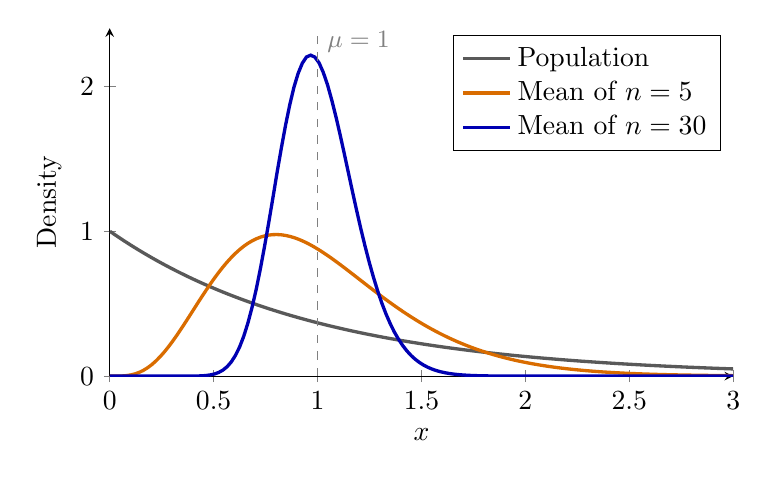
\begin{tikzpicture}
  \begin{axis}[
    width=9.5cm, height=6cm, domain=0.001:3, samples=150, xmin=0, xmax=3, ymin=0, ymax=2.4,
    axis lines=left, xlabel=$x$, ylabel={Density}, legend cell align=left,
    every axis plot/.append style={very thick},
  ]
    % The mean of n draws from Exp(1) has the Gamma(n, rate n) density; the constant for n = 30 is 30 ln 30 - ln 29! = 30.7789.
    \addplot[gray!70!black] {exp(-x)};
    \addplot[orange!85!black] {3125/24*x^4*exp(-5*x)};
    \addplot[blue!70!black] {exp(30.7789 + 29*ln(x) - 30*x)};
    \draw[dashed, gray] (axis cs:1,0) -- (axis cs:1,2.4) node[pos=0.96, right, font=\small] {$\mu = 1$};
    \legend{Population, Mean of $n = 5$, Mean of $n = 30$}
  \end{axis}
\end{tikzpicture}
